\begin{theo}[Elektromagnetische inductie]{Elektromagnetische inductie}
    Een spoel, X, was verbonden aan een batterij. De stroom die door X gaat produceert een magnetisch veld dat versterkt
    wordt door de ijzere kern. De tweede spoel Y werd verbonden aan een galvanometer. De hoop was nu om door magnetisme 
    een stroom te verkrijgen in Y. De constructie is hieronder uitgebeeld
    
    \begin{center}
        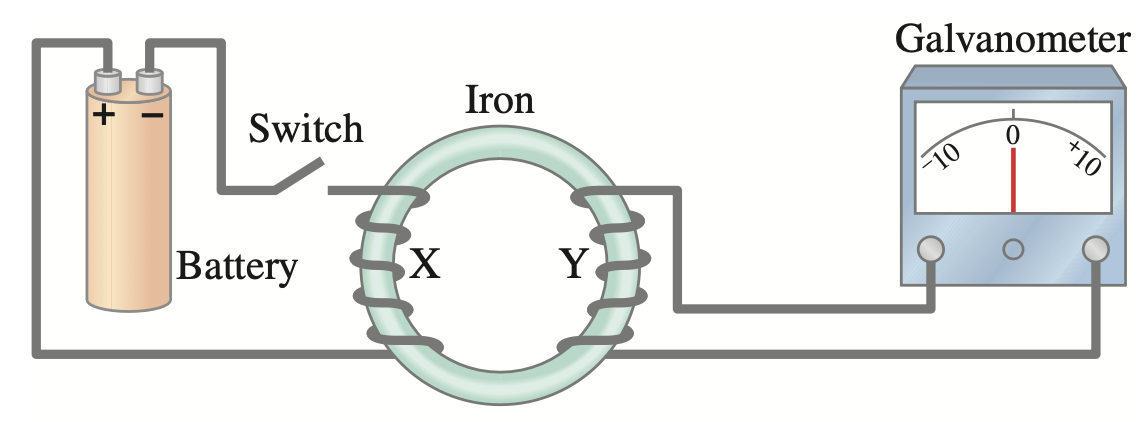
\includegraphics[scale = 0.35]{Images/Magnetisme/MagnetischeInductieExperiment.png}
    \end{center}

    \noindent Als we nu de schakelaar open zouden doen, waardoor X niet meer verbonden zou zijn met de batterij en dus geen stroom meer zou bevatten, 
    dan zou de galvanometer een \textbf{geïnduceerde stroom} weergeven. Dit gebeurt ook op het moment waarop we de schakelaar dicht doen, waarbij het
    magnetisch veld dus verandert. We concluderen: wanneer het magnetisch veld door Y verandert, komt er een stroom voor alsof Y verbonden zou 
    zijn met een emf. Kortom, een veranderend magnetisch veld induceert een emf. Dit fenomeen wordt \textbf{elektromagnetische inductie} genoemd. 
    Omgekeerd, we kunnen ook een magneet snel nabij een geleider brengen. Hierdoor zal er dus een stroom geïnduceerd worden in de geleider.
    De figuur hieronder beeld drie situaties uit, namelijk
    \begin{enumerate}[(a)]
        \item Magneet wordt snel bij een draad gebracht
        \item Magneet wordt snel bij een draad weggehaald
        \item Magneet wordt stilgehouden bij een draad
    \end{enumerate}

    \begin{center}
        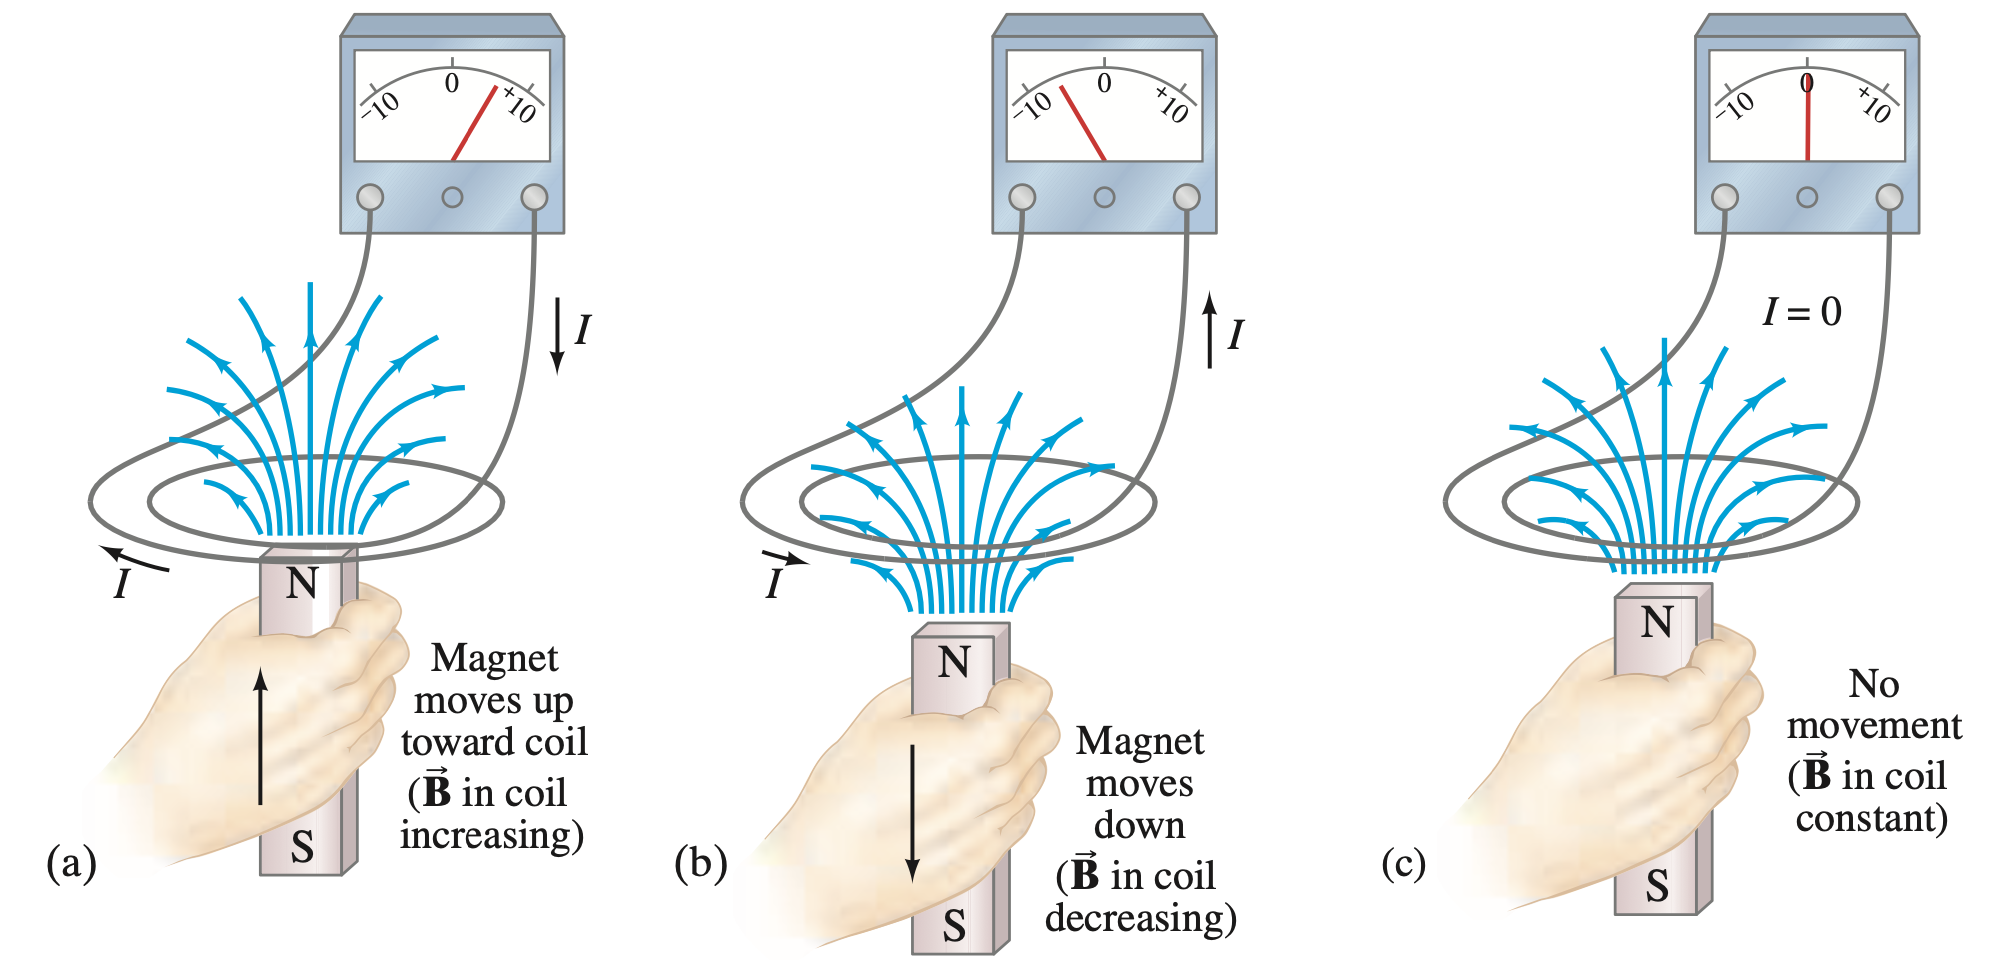
\includegraphics[scale = 0.35]{Images/Magnetisme/MagnetischeInductieMagneet.png}
    \end{center}
\end{theo}

\newpage

\begin{theo}[Magnetische flux]{Magnetische flux}
    \vspace{-0.65cm}
    \begin{minipage}{0.75\textwidth}
        Magnetische flux, net zoals elektrische flux, wordt gedefinieerd als de hoeveelheid magnetisch veld dat door een oppervlakte vloeit.
        Dit komt dan overeen met de formule 
        \begin{equation*}
            \Phi_{B} = \oint \Vec{B} \cdot d\Vec{A}
        \end{equation*}
    \end{minipage}
    \begin{minipage}{0.21\textwidth}
        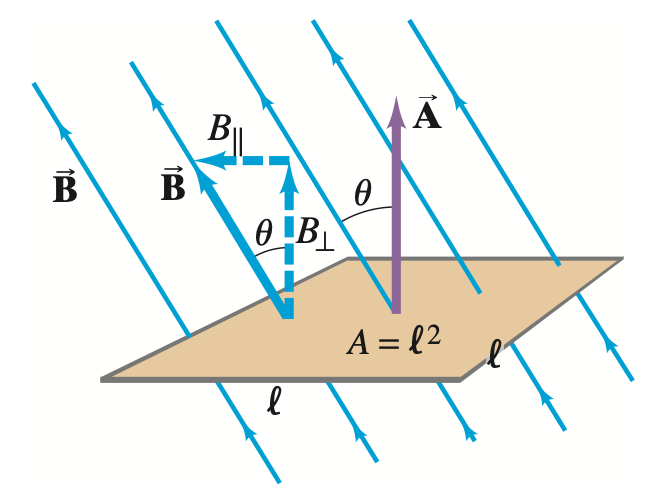
\includegraphics[scale=0.35]{Images/Magnetisme/Faraday.png}
    \end{minipage}
    \vspace{-0.15cm}
\end{theo}
    
\begin{lem}[Faraday]{Faraday}
    De geïnduceerde emf in een gesloten circuit is gelijk aan minus de tijdsverandering van de magnetische flux doorheen de kring met $N$ windingen,
    waardoor dezelfde magnetische flux gaat, in formulevorm:
    \begin{equation*}
        \mathcal{E_{\text{ind}}} = -N\dfrac{d\Phi_{B}}{dt}
    \end{equation*}
    % Als een circuit N windingen heeft die dicht bij elkaar zijn zodat dezelfde flux door elke winding gaat, dan kan je de geïnduceerde spanningen
    % optellen. We krijgen
    % \begin{equation*}
    %     \mathcal{E} = - N \dfrac{d\Phi_{B}}{dt}
    % \end{equation*}
    Het minteken dient als herinnering voor de richting van de geïnduceerde spanning.
\end{lem}

\begin{lem}[Lenz]{Lenz}
    De stroom geproduceerd door een geïnduceerde emf beweegt in een richting zodat het magnetisch veld geproduceerd 
    door die stroom de verandering in magnetische flux doorheen het oppervlak tegenwerkt. We spreken nu over twee distincte velden, namelijk
    \begin{enumerate}
        \item het veranderend magnetisch veld of flux die de stroom induceert
        \item het magnetisch veld geproduceerd door de geïnduceerde stroom
    \end{enumerate}
    waarbij het tweede veld het eerste tegenstelt. Als dit niet zo zou zijn, dan zou er een kettingreactie zijn van
    geïnduceerde emf's en stromen. Dit is in tegenspraak met de wet van behoud van energie.
\end{lem}

\begin{app}[Geïnduceerde emf in een bewegende geleider]{Geïnduceerde emf in een bewegende geleider}
    \begin{minipage}{.69\textwidth}
        We kunnen ook op een andere manier een emf induceren, namelijk met een bewegende geleider. Stel je een uniform magnetisch veld
        $\Vec{B}$ loodrecht is met de oppervlakte van de U-vormige geleider en de bewegende staaf op de geleider ligt (en er dus een kring 
        ontstaat). Als de rod beweegt met een snelheid $v$, dan legt het een afstand $dx = vdt$ af in een tijd $dt$.  Dus vergroot de oppervlakte
        van de kring met $dA = \ell dx = \ell v dt$ in een tijd $dt$. Volgends de wet van Faraday is er nu een geïnduceerde emf
    \end{minipage}
    \begin{minipage}{.27\textwidth}
        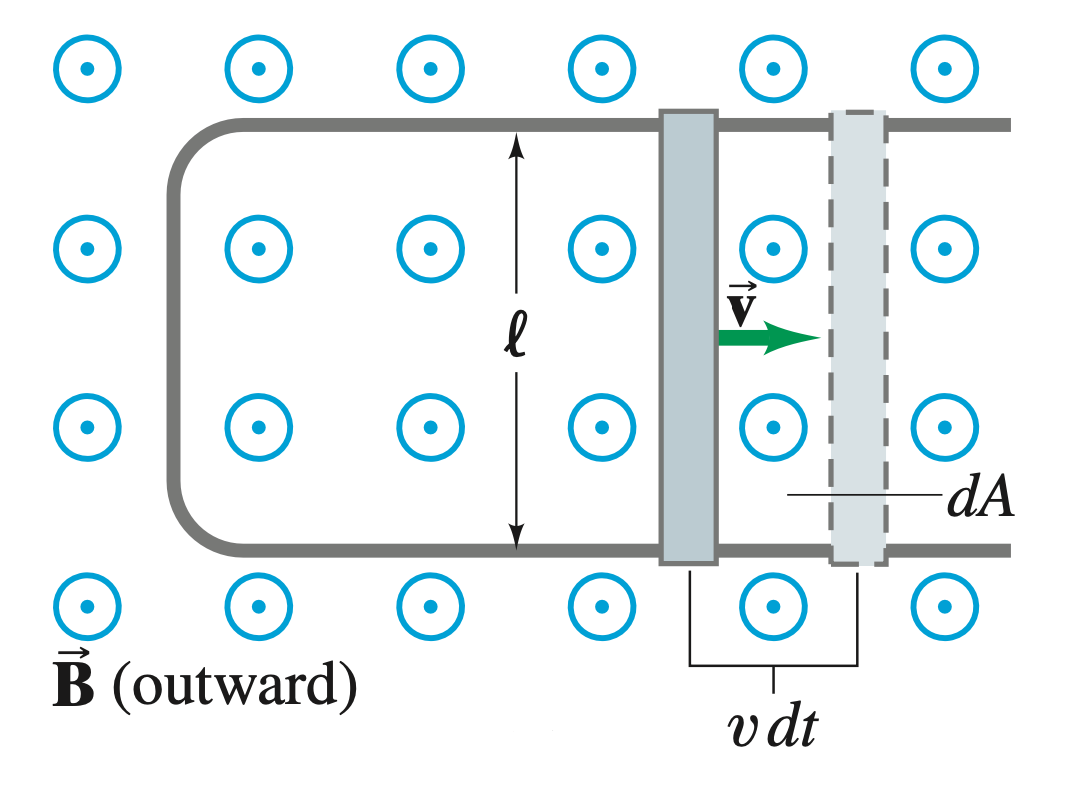
\includegraphics[scale = 0.23]{Images/Magnetisme/BewegendeGeleider}
    \end{minipage}
        \begin{equation*}
            \mathcal{E} = \dfrac{d\Phi_{B}}{dt} = \dfrac{BdA}{dt} = \dfrac{B\ell v dt}{dt} = B \ell v
        \end{equation*}
    waarbij we aannemen dat $B$, $\ell$ en $v$ onderling loodrecht zijn. Als dit niet zo is, dan gebruiken we de loodrechte componenten.
\end{app}

\newpage

